\documentclass{article}

\usepackage{graphicx}
\usepackage{float}
\usepackage{indentfirst}
\usepackage[a4paper, total={6in, 8in}]{geometry}
\usepackage{hyperref}
\usepackage{fancyhdr}
\usepackage{xepersian}
\settextfont{B Nazanin}
\setlatintextfont{Times New Roman}

\begin{document}


%title page%
\begin{titlepage}
	\begin{center}
		\textbf{ \Huge{به نام خدا}}
	
		\vspace{0.2cm}
		
		
\includegraphics[width=0.4\textwidth]{sharif.png}\\
		\vspace{0.2cm}
		\textbf{ \Huge{آزمایش شماره 5}}\\
		\vspace{0.25cm}
		\textbf{ \Large{آز معماری - دکتر سربازی آزاد}}
		\vspace{0.2cm}
		
		
		\large \textbf{دانشکده مهندسی کامپیوتر}\\\vspace{0.1cm}
		\large   دانشگاه صنعتی شریف\\\vspace{0.2cm}
		\large   ﻧﯿﻢ‌سال اول ۰۰-۰۱ \\\vspace{0.10cm}
		\large{ گروه:}\\
		\large{\href{mailto:a.h.hadian@gmail.com}{امیرحسین هادیان - ۹۷۱۰۲۶۰۹}}\\
		\large{\href{mailto:mofayezi.m@gmail.com}{محمدرضا مفیضی - ۹۸۱۰۶۰۵۹}}\\
		\large{\href{mailto:a.hatam008@gmail.com}{علی حاتمی تاجیک - ۹۸۱۰۱۳۸۵}}\\
	\end{center}
\end{titlepage}
%title page%

\newpage

%pages header
\pagestyle{fancy}
\fancyhf{}
\fancyfoot{}
\setlength{\headheight}{59pt}
\cfoot{\thepage}
\lhead{آزمایش شماره 5}
\rhead{
\includegraphics[width=0.1\textwidth]{sharif.png}\\
		دانشکده مهندسی کامپیوتر
}
\chead{آز معماری}
%pages header

\section{هدف}
هدف از این آزمایش ساخت واحد محاسبات که طراحی آن در دستور کار آمده است خواهد بود.

\section{طراحی}
از آنجایی که طرح کلی داده شده است طراحی خاصی نیاز ندارد. چند چیز کلی طراحی شده اند:
\begin{figure}[H]
	\centering
	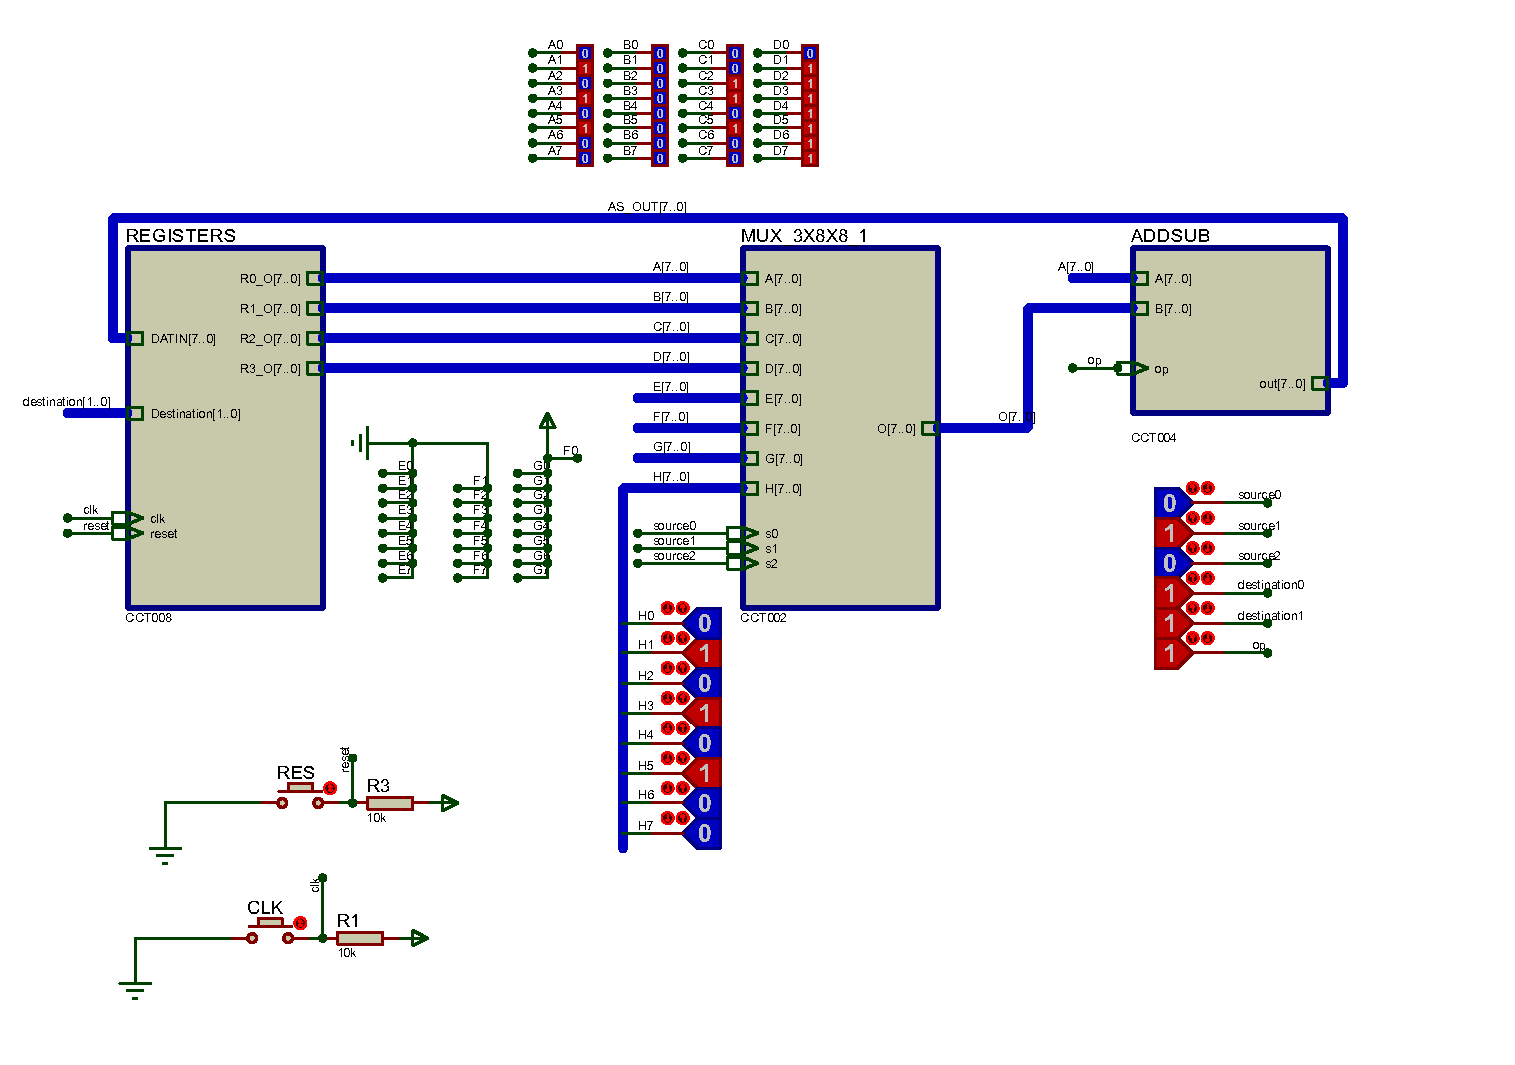
\includegraphics[scale=0.5,page=1]{graphics}
\end{figure}
\subsection{واحد رجیستر}
این بخش خروجی بخش \lr{Adder/Subtractor }را به صورت یک گذرگاه \lr{DATIN} و \lr{destination} که نشان‌دهنده رجیستر مقصد است را ورودی می‌گیرد. همچنین ورودی کلاک و ریست هم برای کنترل رجیسترها داده می‌شود.
ابتدا با توجه به \lr{destination} و یک \lr{decoder} یکی از رجیسترهای \lr{R0} تا \lr{R3} برای لود شدن انتخاب می‌شود. از شیفت رجیستر \lr{74198} برای نگه‌داری \lr{R0} تا \lr{R3} استفاده شده که ورودی \lr{S0} و \lr{S1} آن هردو به خروجی دیکودر وصل شده تا فقط درصورت لزوم مقداردهی شوند. (باتوجه به دیتاشیت تراشه زمانی که هردو \lr{S} صفر باشند کاری انجام نمی‌شود و وقتی هردو یک باشند لود صورت می‌گیرد)
در نهایت خروجی این ماژول طبق مدار به ماتلیپلکسر اصلی داده می‌شود.
\begin{figure}[H]
	\centering
	\includegraphics[scale=0.5,page=4]{graphics}
\end{figure}
\subsection{مالتی‌پلکسر}
مالتی‌پلکسر ۸ به ۱:
این قطعه ۸ ورودی ۸ بیتی گرفته و با توجه به بیت‌های انتخاب، ورودی مورد نظر را در خروجی بارگزاری می‌کند.
برای ساخت این مالتی‌پلکسر از یک طراحی پایین به بالا عمل کردیم و با ساخت یک مالتی‌پلکسر ۲ به ۱، یک مالتی‌پلکسر ۴ به ۱ ساختیم و سپس به کمک آن، مالتی‌پلکسر نهایی را طراحی کردیم.

\begin{figure}[H]
	\centering
	\includegraphics[scale=0.5,page=2]{graphics}
\end{figure}
\begin{figure}[H]
	\centering
	\includegraphics[scale=0.5,page=6]{graphics}
\end{figure}
\begin{figure}[H]
	\centering
	\includegraphics[scale=0.5,page=7]{graphics}
\end{figure}

\subsection{جمع‌کننده و تفریق کننده}
در این بخش دو ورودی \lr{A} و \lr{B} گرفته می‌شوند که با توجه به نوع \lr{op} (0 به معنای عمل جمع و یک عمل تفریق) عملیات انجام داده می‌شود. برای انجام تفریق همه بیت‌های \lr{B }با \lr{op} ایکس‌اور شده تا مکمل دو آن هنگام عمل تفریق بدست آید. برای انجام عملیات نیز از دو جمع‌کننده 4 بیتی استفاده شده که \lr{cout} اولی \lr{cin} دومی قرار گرفته است. (به روش \lr{cascade} یک جمع‌کننده \lr{8} بیتی ساختیم)
\begin{figure}[H]
	\centering
	\includegraphics[scale=0.5,page=3]{graphics}
\end{figure}
\section{تست}
برای تست مدار به این صورت عمل می‌کنیم که ابتدا از ورودی مالتیپلکسر که رزرو بود و جمع آن با رجیستر \lr{R0} که در ابتدا صفر است جمع زده و در رجیستر مقصد می‌ریزیم زمانی که داده‌های تست در رجیسترها لود شدند با زدن یک کلاک (برای تست مدار و لود عددها از کلاک اتوماتیک استفاده نشده است و کلاک به صورت پوش باتن مورد استفاده قرار گرفته است) نتیجه در رجیستر مقصد ریخته خواهد شد.
برای تست ابتدا عدد \lr{101100} را در ریجستر شماره ۲ و پس از آن عدد \lr{101010} را در رجیستر صفر لود می‌کنیم و سپس به تست می‌پردازیم.

\subsection{تست جمع}
\begin{figure}[H]
	\centering
	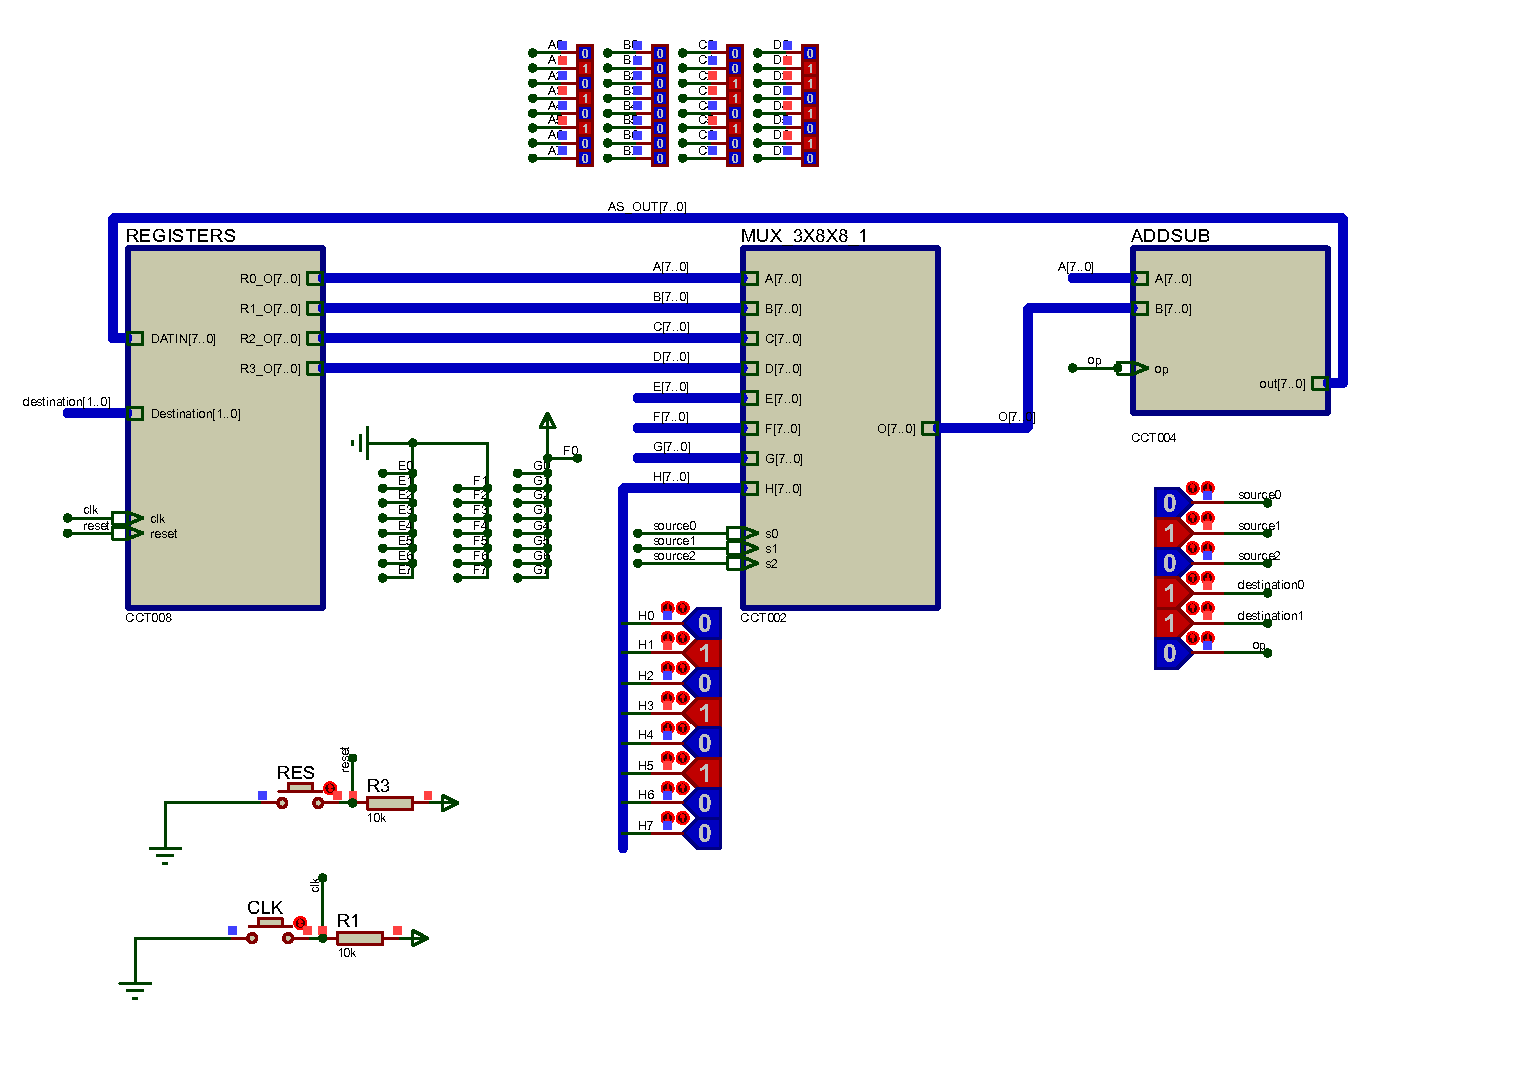
\includegraphics[scale=0.5]{testadd}
\end{figure}
\subsection{تست تفریق}
\begin{figure}[H]
	\centering
	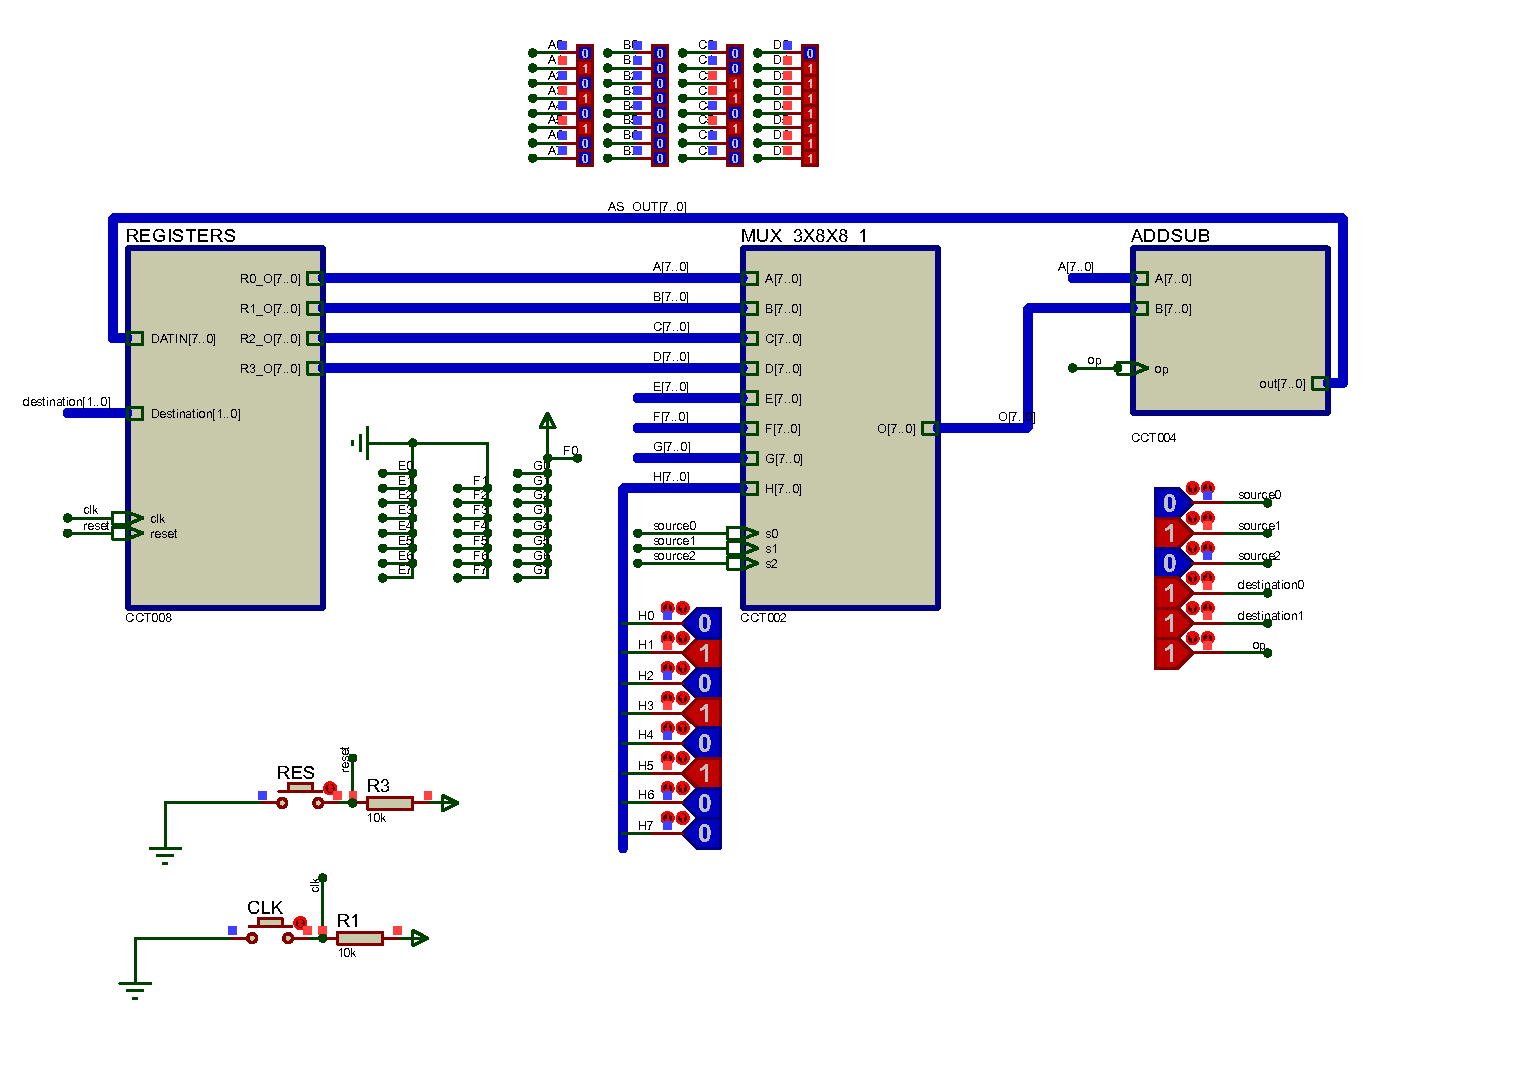
\includegraphics[scale=0.5]{testsub}
\end{figure}
\end{document}
